\chapter{Análisis y estado del arte}
\label{chap:analisis_estado_arte}

\lettrine{C}{omo} ya se comentó en la introducción, la inteligencia artificial está en auge tanto en el mundo académico como, cada vez más, en el \textit{mainstream}. Fruto de 

\textbf{TODO RELOCATE}

\section{Últimos avances y tecnologías}
\label{sec:ultimos_avances_tecnologias}
Los últimos avances en \acrshort{ia} vienen principalmente determinados por una palabra concreta: \textit{transformer}. Y es que este tipo de redes neuronales, capaces de mantener cierto nivel de atención \cite{vaswani2017attention_all_you_need} durante su funcionamiento, han sido las causantes de una fiebre en la que compañías como OpenAI, Google, Meta o incluso Tesla se han lanzado a realizan amplias inversiones en el campo. Dichas compañías y multitud de investigadores sorprenden todos los años con modelos innovadores, rompiendo la barrera de lo que se creía posible hasta el momento.

Algunas de las arquitecturas basadas en \textit{transformers} más relevantes son AlphaFold para el plegado de proteínas, Tesla Autopilot para conducción autónoma, GPT-3 para la generación de texto, DALL$\cdot$E 2 para generación de verdaderas obras de arte, así como la reciente red generalista GATO, entre otros.

Estos transformers, además, pueden aplicarse a arquitecturas ya existentes como las \textit{\acrshort{gan}}s (\textit{\acrlong{gan}})\footnote{\url{https://en.wikipedia.org/wiki/Generative\_adversarial\_network}} para obtener resultados visiblemente espectaculares, como se puede observar en la Figura \ref{fig:vqgan_image}, o en el proyecto \cite{chang2022maskgit}, donde se emplean transformers y \textit{VQGAN}s para realizar todo tipo de manipulaciones sobre imágenes.

\begin{figure}[h!]
    \centering
    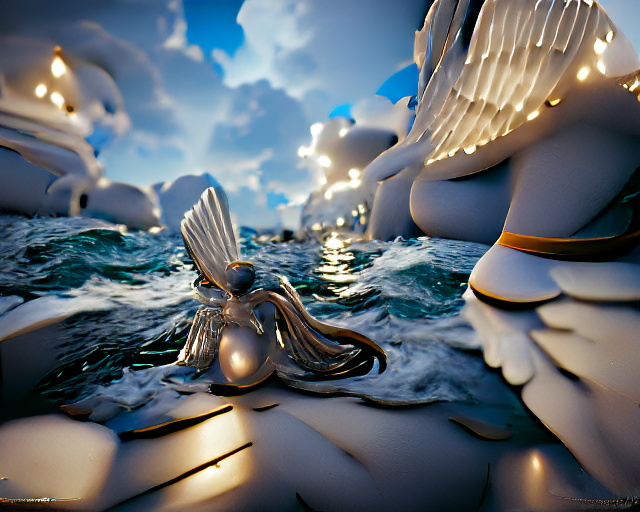
\includegraphics[width=0.8\textwidth]{img/vqgan_image.png}
    \caption{Arte generado por redes \textit{GAN} complementadas con \textit{transformers}}
    \label{fig:vqgan_image}
\end{figure}

\section{Requerimientos energéticos de las redes neuronales}
\label{sec:requerimientos_energeticos_redes_neuronales}
Las cada vez más increíbles capacidades de las redes neuronales artificiales no vienen sin coste. El coste de personal de investigación y desarrollo, así como el coste energético del proceso de entrenamiento siguen siendo exageradamente altos para proyectos complejos como los citados en la sección anterior.

Sin embargo, en este trabajo no se trata el proceso de desarrollo y entrenamiento, ya que eso se delega en los numerosos y muy competentes ingenieros en inteligencia artificial. En este trabajo se trata el proceso de inferencia, es decir, la ``ejecución'' de una red creada y entrenada.

El proceso de inferencia es mucho más sencillo y computacionalmente menos demandante que el de entrenamiento, pero tras esa falsa sensación de ``gratuidad'' de bajos recursos computacionales se oculta una trampa en la escala de dichos recursos. Esto es debido a que, a pesar de que una red neuronal durante el proceso de desarrollo se entrena múltiples veces con un elevado coste asociado, este entrenamiento es habitualmente llevado a cabo por un pequeño grupo de ingenieros. Por otro lado, si bien la ejecución de redes neuronales es mucho más barata computacionalmente hablando, la escala de estas redes neuronales, especialmente de las que aspiran a convertirse en parte de nuestras vidas, hace que un consumo de unos pocos mWh se convierta en varios kWh o incluso MWh por dispositivo a lo largo de todo el planeta.

Añadiendo a esto que se pretende que en el futuro prácticamente cualquier bien de consumo tenga inteligencia artificial asociada, la demanda de energía pasa a ser una preocupación importante, en la escala de los TWh. Es debido a esto que una reducción del 10\% del consumo, a pesar de parecer un logro menor, es muy importante para la sostenibilidad a largo plazo de nuestro planeta y estilo de vida.

\section{Investigación y optimizaciones propuestas}
\label{sec:investigacion_optimizaciones_propuestas}
Como ya se comentó en la Sección \ref{sec:redes_neuronales}, la multiplicación de matrices es parte fundamental e imprescindible de la ejecución de redes neuronales no convolucionales. Esto se puede visualizar mejor en la Figura \ref{fig:profiling_several_nns}, donde se muestra en qué cargas de trabajo se invierten más ciclos en varias redes neuronales de referencia \cite[Figura 3.4]{deep_learning_for_computer_architects}. Como es de esperar, en las redes que no requieren de convolución para su funcionamiento, el porcentaje del tiempo que se dedica a la multiplicación de matrices es muy elevada, por lo que atacar dicho punto parece la decisión correcta. Sin embargo, como ingeniero informático, la optimización del algoritmo de multiplicación de matrices generales no parece un campo poco trabajado y abordable para una persona sin formación específica en matemáticas y algoritmia avanzada.

\begin{figure}[h!]
    \centering
    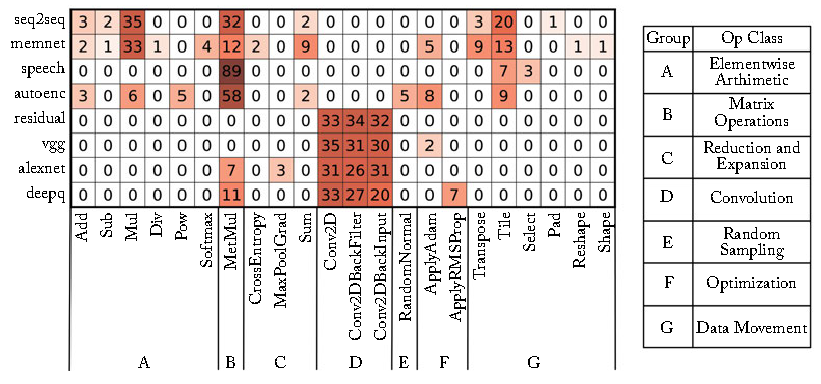
\includegraphics[width=\textwidth]{pdf_tex/dlfca_figure3_4.pdf}
    \caption{Tiempo empleado en funciones (\%) según tipo de red neuronal}
    \label{fig:profiling_several_nns}
\end{figure}

Tras la multiplicación de matrices, las cargas de trabajo más habituales siguen estando relacionadas con el tamaño del modelo, siendo estas operaciones \textit{elementwise}, es decir, que afectan a elementos individualmente, como la multiplcación, suma o división. Por último, otra gran carga de trabajo, y gran fuente de gasto de energía, es el movimiento de datos en memoria.

Solventar estos problemas no es tarea trivial. Ignorando la cada vez menos presente Ley de Moore, mediante la cual los microchips tienden a ser cada vez más pequeños, y por tanto más eficientes energéticamente, una reducción o estancamiento en el tamaño de las redes no es una solución asumible. Sin embargo, que las redes no se puedan reducir en tamaño manteniendo el mismo esquema de conexiones denso no implica que no se pueda conservar el tamaño de la red, alterando el esquema de conexiones. Es aquí donde las redes neuronales dispersas comienzan a destacar como una opción con menor número de FLOPs, y por tanto con menor consumo teórico de energía.

\subsection{Podado y redes dispersas}
\label{ssec:podado_y_redes_dispersas}
Mediante el proceso de podado, una red neuronal puede ver enormemente mejorado su rendimiento a costa de pequeños descensos en la precisión hasta cierto umbral. Encontrar este \textit{sweet-spot} es crucial si se desea una implementación competente, pero a la vez lo más eficiente posible. En la Figura \ref{fig:grafica_sparse_vs_dense} \cite{neuralmagic_pruning_overview} se puede apreciar cómo la precisión va progresivamente cayendo a medida que el rendimiento aumenta.

\begin{figure}[h!]
    \centering
    \vspace*{0.5cm}
    \def\svgwidth{0.9\textwidth}
    \input{pdf_tex/grafica_sparse_vs_dense/grafica_sparse_vs_dense.pdf_tex}
    \caption{Comparación de rendimiento y precisión con una red neuronal dispersa}
    \label{fig:grafica_sparse_vs_dense}
\end{figure}

Como se puede apreciar, en el correcto podado de redes neuronales se puede encontrar una posible solución a la elevada potencia de cómputo necesaria para la ejecución de las mismas. Sin embargo, el podado solamente ofrece resultados extraordinarios con precisiones extraordinariamente bajas. Este comportamiento sin embargo no debe ser desmotivador, puesto que con las herramientas, profesionales e investigación adecuada, estas tecnologías basadas en redes neuronales dispersas probablemente tengan un amplio margen de mejora mediante optimizaciones, arquitecturas y procesos de entrenamiento específicos.

\subsection{XPU: \textit{X Processing Unit}}
\label{ssec:xpu}
Otra posible vía de mejora de esta eficiencia es mediante la creación de circuitos de aplicación específica para inferencia, un camino muchísimo más barato de señalar que de realizar.

Un circuito de aplicación específica o \acrshort{asic} (\textit{\acrlong{asic}}) por sus siglas en inglés es probablemente lo más alto que se puede llegar en cuanto a eficiencia de cómputo de un \textit{workload}, pero también es lo que incurre en más gastos derivados de su desarrollo. Estos costes se sitúan en los (miles de) millones de euros, y el proceso de diseño es especializado, costoso, y muy punitivo si se descubren errores graves en el diseño. Es por esto que diseñar un \acrshort{asic} para inferencia es una tarea al alcance de muy pocos.


Sin embargo, esto no ha frenado a los grandes en el universo de la \acrshort{ia} en su afán por más rendimiento y flexibilidad. Circuitos como la \acrshort{tpu} (\textit{\acrlong{tpu}}) de Google son ya una realidad. En la Figura \ref{fig:tpu_block_diagram} \cite{jouppi2017_in_datacenter_tpu} se puede ver el diagrama de bloques del chip TPU. En esta imagen se puede ver cómo un componente principal de dicho chip es el multiplicador de matrices. Este componente (entre otros) hace que esta pieza de hardware tenga un rendimiento y eficiencia muy superiores a sus contrapartes \acrshort{cpu} y \acrshort{gpu}, como se puede observar en la Figura \ref{fig:tpu_benchmarks} \cite{devopedia_tpu}.

\begin{figure}[h!]
    \centering
    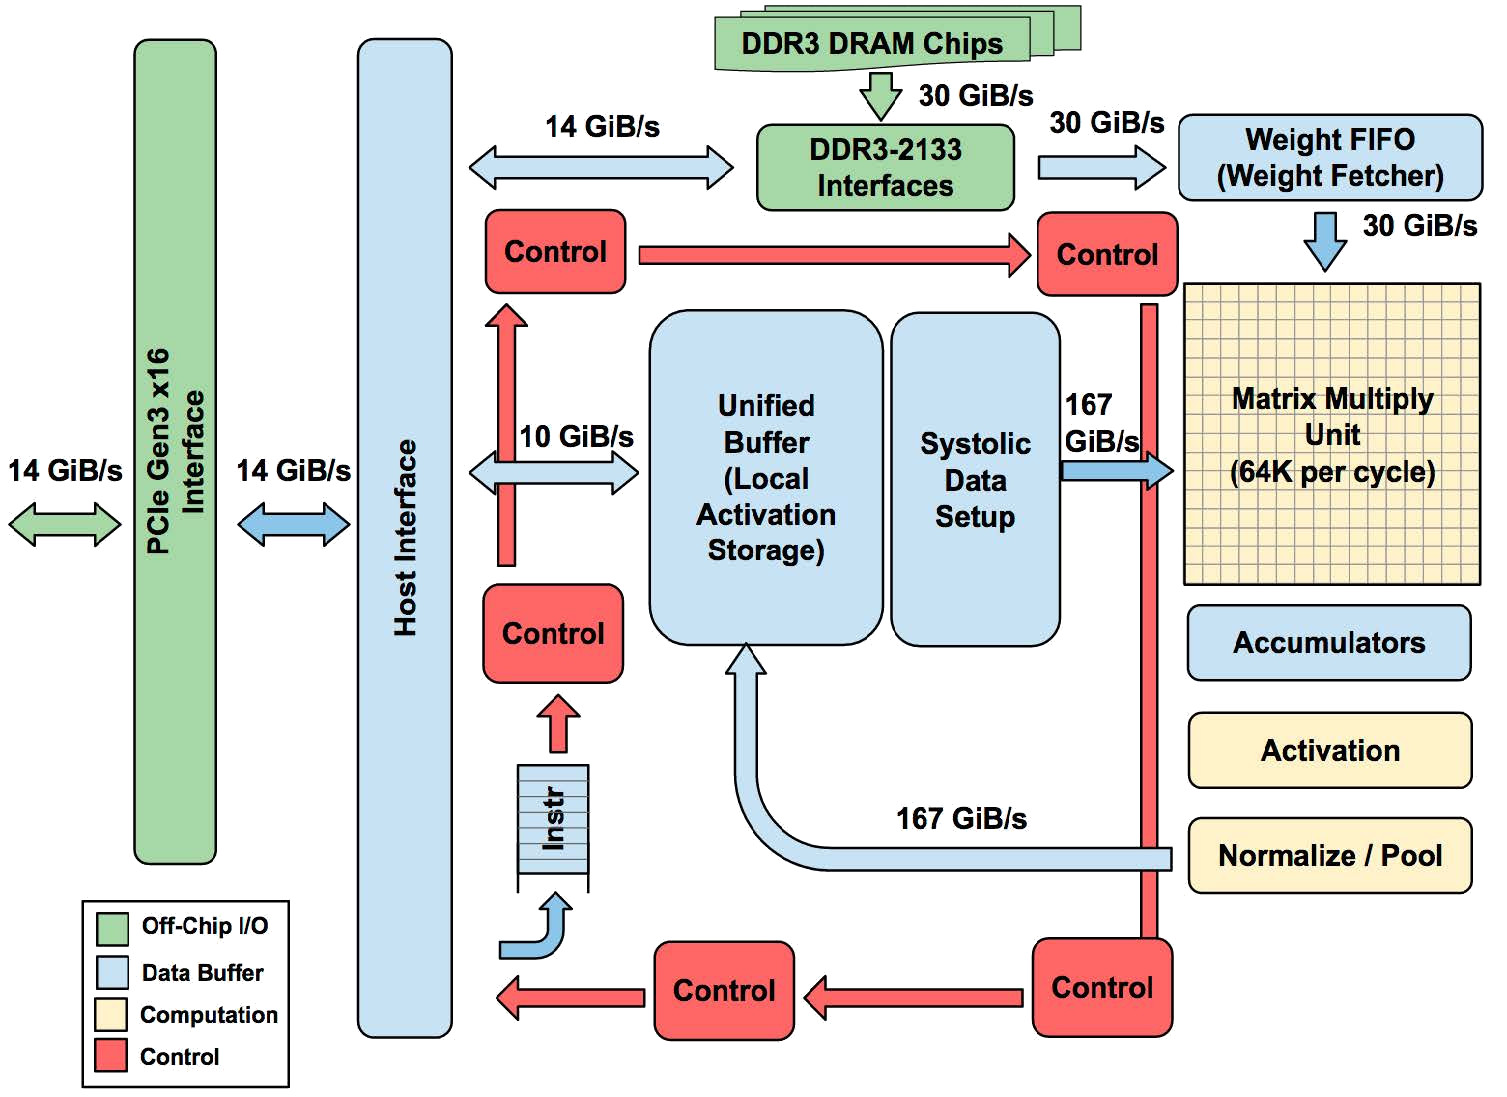
\includegraphics[width=0.85\textwidth]{img/tpu_block_diagram.jpg}
    \caption{Diagrama de bloques del chip TPU de Google}
    \label{fig:tpu_block_diagram}
\end{figure}

\begin{figure}[h!]
    \centering
    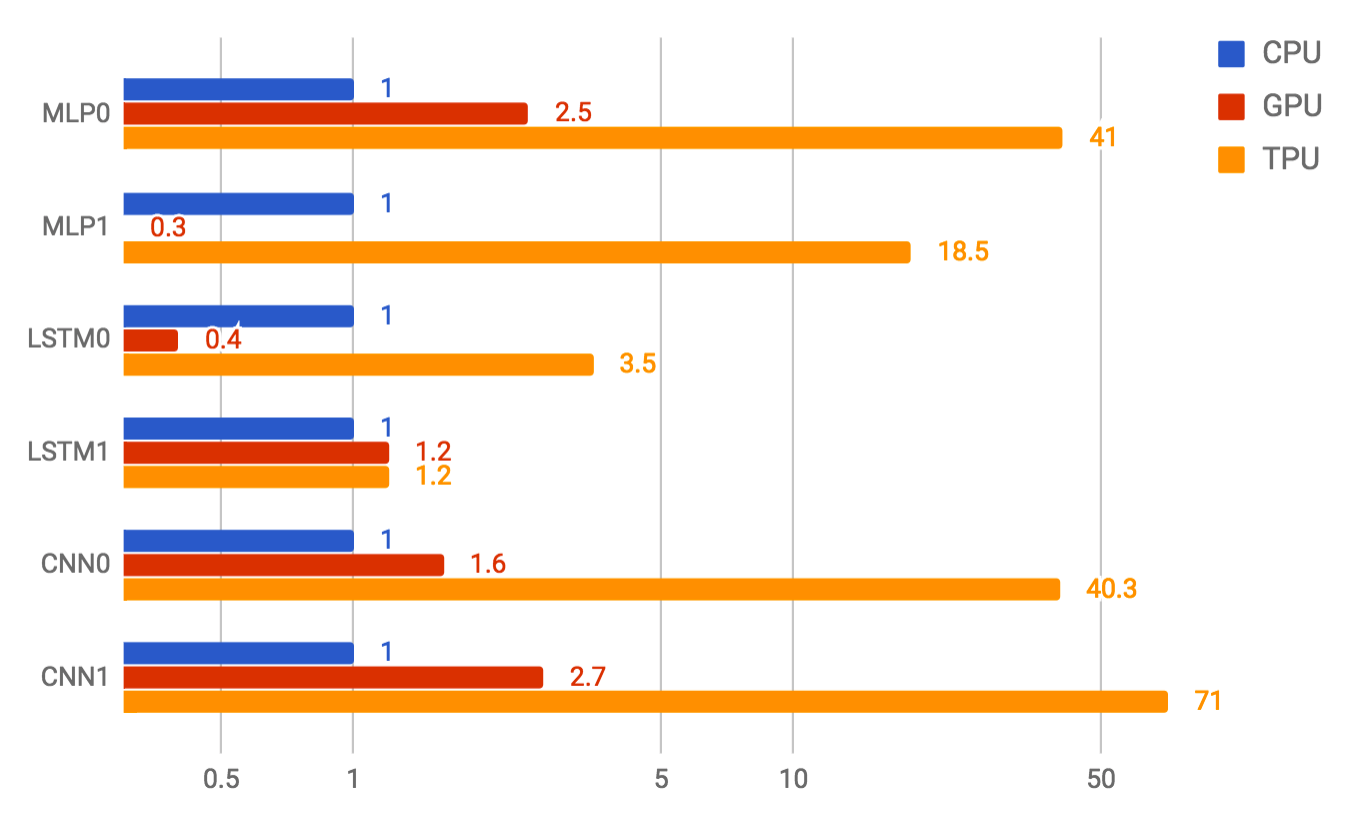
\includegraphics[width=0.85\textwidth]{img/tpu_benchmarks.png}
    \caption{Resultados del chip TPU de Google en comparativa con otras alternativas}
    \label{fig:tpu_benchmarks}
\end{figure}

\subsection{Otras optimizaciones}
\label{ssec:otras_optimizaciones}
Existen también otras optimizaciones como el uso de DRAM aproximada. Estas son redes neuronales re-entrenadas sobre una plataforma con DRAM que pueda incurrir en fallos en la transferencia de datos, las cuales pueden aprender a identificar estos errores y adaptarse a ellos, usando tanto mecanismos explícitamente diseñados para ello, como de forma automática \cite{deep_learning_for_computer_architects} \cite{koppula2019eden}. Si bien esta aproximación reduce la precisión de la red (de igual forma que lo hacen las previamente discutidas) el ahorro de energía en accesos a memoria, que supone gran parte del consumo total de energía en sistemas embebidos, puede marcar la diferencia si se encuentra el equilibro entre precisión y consumo.